\subsection{连续映射的同伦提升条件}

命题 1. --- 设 B 是拓扑空间，(E,p) 是 B 的覆叠。设 Y 是拓扑空间，f: Y → B 是连续映射。设 y ∈ Y、x ∈ E、b ∈ B 满足 f(y) = p(x) = b。假设空间 Y 连通且局部道路连通。要存在满足 g(y) = x 的连续提升 g: Y → E，使其提升 f，必要且充分条件是同态 π₁(f,y): π₁(Y,y) → π₁(B,b) 的像包含于同态 π₁(p,x): π₁(E,x) → π₁(B,b) 的像中。

不对空间 Y 作任何假设，该条件仍是必要的。事实上，若这样的提升 g 存在，则有 \(\pi_{1}(f,y)=\pi_{1}(p,x)\circ\pi_{1}(g,y)\)。

证明它是充分的。记 \(s\colon \Lambda_{b}(\mathrm{B})\to \Lambda_{x}(\mathrm{E})\) 为同胚 \(c\mapsto p\circ c\) 的逆同胚（III，第 302 页，命题 3 的推论 2），并令 \(\varphi \colon \Lambda_y(\mathrm{Y})\to \Lambda_x(\mathrm{E})\) 为映射 \(d\mapsto s(f\circ d)\)。映射 \(\varphi\) 连续（I，第 132 页，引理）。

设 \(d\) 和 \(d' \in \Lambda_y(Y)\) 是起点为 \(y\) 且终点相同的道路；证明道路 \(\varphi(d)\) 和 \(\varphi(d')\) 的终点相同。置 \(c = f \circ d\)、\(c' = f \circ d'\)。由于道路 \(d * \overline{d'}\) 是 Y 中以 \(y\) 为基点的圈，道路 \(c * \overline{c'}\) 是 B 中以 \(b\) 为基点的圈，且其类属于同态 \(\pi_1(f, y)\) 的像，因而根据假设属于同态 \(\pi_1(p, x)\) 的像。由命题 4 的推论 2（III，第 303 页），道路 \(s(c * \overline{c'})\) 是 E 中以 \(x\) 为基点的圈。道路 \(s(c' * \overline{c})\) 也如此；由道路提升的唯一性，它等于 \(\overline{s(c * \overline{c'})}\)。因此有 \(s(c' * \overline{c})(\frac{1}{2}) = s(c')(1) = s(c)(1)\)，这正是要证明的。

分别记 \(e_{\mathrm{E}}\colon\Lambda_{x}(\mathrm{E})\to\mathrm{E}\) 和 \(e_{\mathrm{Y}}\colon\Lambda_{y}(\mathrm{Y})\to\mathrm{Y}\) 为终点映射。由于假设空间 Y 连通且局部道路连通，映射 \(e_{Y}\) 是满射且开（III，第 262 页，命题 10）。由上一段，存在唯一的映射 \(g\colon Y\to E\)，使得 \(e_{E}\circ\varphi=g\circ e_{Y}\)。它是连续的，因为映射 \(e_{Y}\) 是严格映射（I，第 18 页，例 2）。

最后，验证映射 g 提升映射 f 且 \(g(y) = x\)。Y 的每一点 z 都是一条起点为 y 的道路 c 的终点。道路 \(\varphi(c)\) 是 \(f \circ c\) 的、起点为 x 且终点为 \(g(z)\) 的提升。因此有 \(p(g(z)) = f(z)\)。当 z = y 且 \(c = e_y\) 时，有 \(\varphi(e_y) = e_x\)，从而 \(g(y) = x\)。

推论 1. --- 设 B 是连通且局部道路连通的拓扑空间，b 是 B 的一点。要使 B 的覆叠 (E, p) 可平凡化，必要且充分条件是：对于纤维 \(E_{b}\) 的每一点 x，同态 \(\pi_{1}(p, x)\) 都是双射。

回顾同态 \(\pi_{1}(p,x)\) 是单射（III，第 303 页，命题 4 的推论 1）。因此，该断言由命题 1 以及 I，第 81 页，命题 6 的推论 4 得出。

注记。--- 设 B 是局部道路连通的拓扑空间，b 是 B 的一点，V 是 b 的开连通邻域，并且从 \(\pi_{1}(V,b)\) 到 \(\pi_{1}(B,b)\) 的同态的像是约化为单位元的子群。由推论 1，B 的每个覆叠在 V 上都可平凡化，因而在 B 的每个包含于 V 的子集上也可平凡化。

推论 2. --- 设 B 是连通且局部道路连通的拓扑空间。若对 B 的某一点 b，群 \(\pi_1(B,b)\) 约化为单位元，则空间 B 单连通。

事实上，由推论 1 立即得到，在这些假设下，B 的每个覆叠都可平凡化。

推论 3. --- 设

\pandocbounded{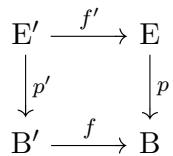
\includegraphics[keepaspectratio]{images/part002_b7191fdb.jpg}}

为笛卡尔方块。假设 E 是 B 的覆叠，且空间 B' 连通并局部道路连通。设 b' 是 B' 的一点，且 \(b = f(b')\)。要使 \((\mathrm{E}', p')\) 成为 B' 的可平凡化覆叠，必要且充分条件是：对于纤维 \(E_b\) 的每一点 x，\(\pi_1(p, x)\) 的像包含 \(\pi_1(f, b)\) 的像。

这由命题 1 以及 I，第 81 页，命题 6 的推论 5 得出。

